\documentclass[11pt]{article}
\usepackage[T1]{fontenc}
\usepackage[utf8]{inputenc}
\usepackage{lmodern}
\usepackage[margin=1in]{geometry}
\usepackage{amsmath,amssymb,amsthm,booktabs,graphicx}
\usepackage{microtype}
\usepackage[round,authoryear]{natbib}
\usepackage{enumitem}
\usepackage{placeins}
\usepackage[colorlinks=true,linkcolor=blue,citecolor=blue,urlcolor=blue]{hyperref}
\setlength{\parskip}{3pt}
\setlength{\parindent}{1em}
\setlist{nosep}
\newtheorem{proposition}{Proposition}
\newcommand{\R}{\mathbb R}
\newcommand{\Cproj}{\mathcal C}
\newcommand{\norm}[1]{\left\lVert#1\right\rVert}
\newcommand{\Frob}{\mathrm F}
\newcommand{\acc}{\mathrm{Acc}}
\DeclareMathOperator{\RMS}{RMS}
\DeclareMathOperator{\diag}{diag}
\DeclareMathOperator{\argmax}{argmax}
\title{Sign Interactions at Fixed Spectral Amplitudes:\\Predicting and Intervening on RFM Initialization\\under a Symmetry Fixed-Point Split}
\author{Xiao Tian}
\date{September 7, 2026}
\hypersetup{pdftitle={Sign Interactions at Fixed Spectral Amplitudes: Predicting and Intervening on RFM Initialization under a Symmetry Fixed-Point Split},pdfauthor={Xiao Tian}}
\begin{document}
\maketitle
\begin{abstract}
We study whether relative Fourier signs in an RFM initialization affect generalization on modular addition, training on unequal input pairs and testing on equal pairs. On 30 prespecified directions, favorable signs improve accuracy by 11.86 percentage points relative to distance-matched random controls (95\% post hoc seed-cluster bootstrap interval [7.15, 17.03]). The effect is larger at modulus 17 (+15.69 points, 20 directions) than at modulus 23 (+4.20 points, 10 directions). Favorable and unfavorable sign optimizations yield 97.6\% and 4.0\% mean accuracy at identical spectral amplitudes and residuals; these are two optimized extremes, not a baseline-to-treatment improvement. Selection uses a finite-amplitude quadratic response tensor. Frozen accuracy forecasts on 50 new directions at modulus 17 and 30 at modulus 23 have mean absolute errors of 4.2 and 6.6 points. Local equivariance restricts linear sector coupling but does not explain quadratic dominance after 59 nonlinear updates. Post hoc analyses quantify continuous-margin error, conditional control gains, tensor structure, and amplitude dependence. Construction cost and parameter sensitivity limit the method's scope.
\end{abstract}

\section{Introduction}
Recursive Feature Machines alternate kernel fitting with an average gradient outer product (AGOP) update of the input metric. For modular arithmetic, this process learns block-circulant features \citep{mallinar2025}. Data symmetries can obstruct generalization, and structured initialization can restore it on a symmetry-preserving split \citep{bernal2026}.

Within this setting, we study which symmetry-breaking directions lead to generalization. In our initial experiments, cross-block perturbations with the same norm succeeded for some directions and failed for others. Diagonal-block perturbations could produce classification collapse. We examine whether these outcomes can be predicted from initialization and altered by controlled interventions.

A local equivariance argument constrains how perturbations enter the circulant cross sector. We then construct a finite-amplitude response tensor to forecast the aligned mean score profile, with a calibration fitted on discovery directions to predict accuracy. The predictor selects sign interventions that preserve every circulant Fourier amplitude and the noncirculant residual. Comparing favorable and unfavorable signs, alongside matched random controls, tests how their relative signs affect the outcome. This prediction and intervention study defines our contribution within the fixed-point split.

\section{Setting and decomposition}\label{sec:setting}
For odd modulus $p$, inputs are $x(a,b)=[e_a,e_b]\in\R^{2p}$ and labels are $y(a,b)=e_{(a+b)\bmod p}$. The training set contains all $n=p(p-1)$ pairs with $a\ne b$; the test set consists of the $p$ pairs $(a,a)$. Each test example therefore has equal weight $1/p$. Accuracy differences are not continuous at the level of an individual direction.

Given a positive semidefinite metric $M$, define
\begin{equation}
 k_M(x,z)=\exp\!\left(-\frac{(x-z)^TM(x-z)}{2\sigma^2}\right),\qquad
 \alpha=K_M^{-1}Y,\qquad f_M(z)=k_M(X,z)^T\alpha .\label{eq:kernel}
\end{equation}
The default bandwidth is $\sigma=2.5$, so the denominator is $12.5$. We use zero ridge regularization. Let $G_i\in\R^{p\times 2p}$ be the input Jacobian of $f_M$ at training point $x_i$, centered across training points. The update is
\begin{equation}
 A_M=\frac1n\sum_{i=1}^n G_i^TG_i,\qquad T(M)=A_M^{1/2},\label{eq:update}
\end{equation}
where the root is the positive semidefinite root. The implementation uses the negative input Jacobian, which gives the same AGOP. All main trajectories have 60 evaluations, indexed $t=0,\ldots,59$, and 59 metric updates. No trace normalization is applied.

Let $P$ exchange the two input blocks. A symmetric swap-odd perturbation satisfies $PEP=-E$ and has the form
\begin{equation}
 E=\begin{pmatrix}A&B\\-B&-A\end{pmatrix},\qquad A^T=A,\quad B^T=-B.
\end{equation}
We call the $A$ part \emph{diag} and the $B$ part \emph{cross}. Initial metrics are
\begin{equation}
 M_0=I+\epsilon\sqrt{2p}\,E,\qquad \norm{E}_{\Frob}=1,\qquad \epsilon=0.01\quad\text{by default}.\label{eq:init}
\end{equation}
All recorded initial metrics are positive definite. Random cross directions are obtained from a seeded Gaussian matrix by symmetrization, swap-odd projection, removal of the diagonal blocks, and Frobenius normalization. The exact generator is included with the code.

Define the circulant projection
\begin{equation}
 (\Cproj B)_{ij}=\frac1p\sum_{r=0}^{p-1}B_{r,\,r+(j-i)\bmod p},\qquad C=\Cproj B,\qquad R=B-C.\label{eq:projection}
\end{equation}
This is an orthogonal projection in the Frobenius inner product, so $C\perp R$. Both are skew-symmetric. For $d=(p-1)/2$, normalized matrices proportional to $\sin(2\pi k(j-i)/p)$, $k=1,\ldots,d$, give an orthonormal basis $E_k$ of the full $2p\times2p$ circulant cross sector. A cross direction decomposes as $E=\sum_k a_k E_k+E_R$. The normalization is on the full matrices, not just their upper-right blocks.

\section{What symmetry explains}\label{sec:theory}
We derive the symmetry constraints in exact arithmetic, with the regularity assumptions stated in each proposition.

\begin{proposition}[Even fixed-point readout]\label{prop:even}
Assume every kernel system along the two trajectories has a unique solution and the metric update uses the unique positive semidefinite root. For a swap-odd direction $E$, the complete test score vector at each fixed point satisfies
\begin{equation}
 F_t(\epsilon;E)=F_t(-\epsilon;E)
\end{equation}
whenever both trajectories are defined.
\end{proposition}
\begin{proof}
Swapping inputs permutes the training examples without changing their labels. Kernel fitting and the AGOP update are equivariant under this orthogonal permutation. Therefore initialization at $PM_0P$ produces $PM_tP$ at every step. Since $Px(a,a)=x(a,a)$, the test scores coincide. Equation~\eqref{eq:init} gives $PM_0(\epsilon)P=M_0(-\epsilon)$.
\end{proof}
Evenness removes odd Taylor coefficients only when those coefficients exist. An even function may contain $|\epsilon|$, and matrix square roots need not be differentiable at singular points. In particular, evenness alone does not prove a quadratic response after many updates.

\begin{proposition}[Conditional local sector selection]\label{prop:selection}
Suppose $T$ is differentiable at a metric $\overline M$ invariant under swap, common cyclic shifts of both input indices, and common index negation. Its derivative $D=T'(\overline M)$ preserves the circulant cross sector. Neither a diag swap-odd direction nor a cross direction with zero circulant projection can have a nonzero circulant cross component after applying $D$.
\end{proposition}
\begin{proof}
Common shifts permute training examples and output classes, as does common negation. The class permutation leaves the AGOP unchanged. Thus $D$ commutes with the corresponding conjugations and with their group averages. Let $\mathcal A$ average conjugation by common shifts; it performs circulant projection on every matrix block. Then $D\mathcal A=\mathcal A D$. For a noncirculant cross residual, $\mathcal A E_R=0$, and hence $\mathcal A D(E_R)=0$.

For a diag direction, $\mathcal A E_{\rm diag}=\diag(\Cproj A,-\Cproj A)$. Let $J$ negate both indices. Conjugation by $J$ transposes a circulant block. A symmetric circulant diagonal block is consequently $J$-even, whereas a skew-symmetric circulant cross block is $J$-odd. Since $D$ preserves $J$ parity, no latter component can be produced by the former. Finally, among symmetric matrices, the common-shift-invariant, swap-odd, $J$-odd sector consists exactly of circulant cross matrices. It is therefore preserved by $D$.
\end{proof}
To quantify the local couplings, we numerically evaluate the analytic derivative of the first update at the initial baseline $I$. The circulant-sector gain is approximately $1.66$ at $p=17$, $1.69$ at $p=23$, and $1.71$ at $p=29$ in the implementation\textquotesingle s absolute metric units. Residual-cross and diag gains are approximately $0.89$--$0.91$ and $0.24$--$0.36$ on the checked directions. These gains describe local perturbation growth at $I$, which is not assumed to be a fixed point of $T$. They do not supply a sufficient condition for classification. Appendix~\ref{app:derivatives} gives the singular-support calculation and its numerical checks.

\begin{figure}[t]
\centering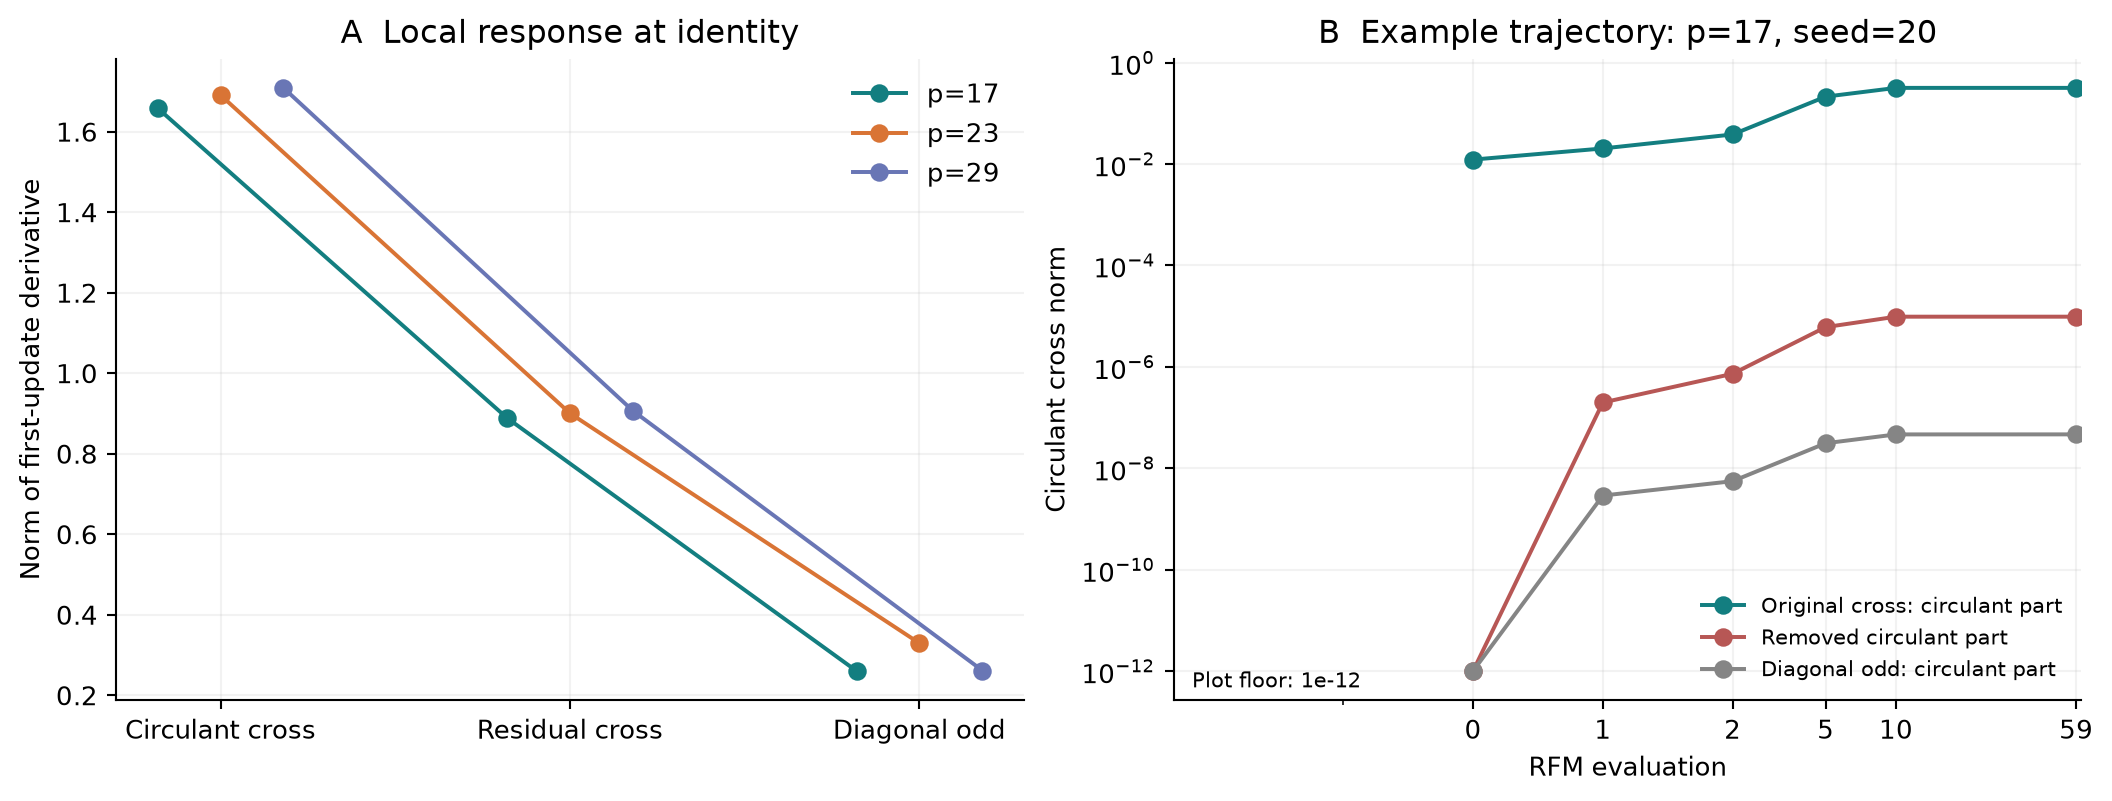
\includegraphics[width=\linewidth]{figures/01_channel_selection.png}
\caption{Numerical derivative gains at the symmetric initial metric and example finite-amplitude trajectories.}\label{fig:channel}
\end{figure}

\begin{proposition}[Pure circulant score profile]\label{prop:profile}
For a pure circulant cross initialization, there is a class-offset profile $v$ such that $F_t(a,a)_c=v_{c-2a\bmod p}$. If the correct offset does not tie for the maximum with an incorrect offset, test accuracy is either zero or one. Moreover, $v_c=v_{-c\bmod p}$.
\end{proposition}
\begin{proof}
Common-shift invariance is preserved by the update. A shift by $a$ sends $(0,0)$ to $(a,a)$ and shifts the label by $2a$, giving the profile relation. Correct predictions correspond to offset zero for every test point. Common negation sends a skew-circulant perturbation $E$ to $-E$ and reverses output offsets. Proposition~\ref{prop:even} identifies the fixed-point outputs of these initializations, giving the last equality.
\end{proof}
Two incorrect offsets may therefore tie. A change in raw argmax between them need not change correctness. General cross initializations also have a noncirculant residual, so their test points can deviate from the mean profile and yield intermediate accuracies. We define that mean profile by
\begin{equation}
 \bar v_c=\frac1p\sum_{a=0}^{p-1} F_{59}(a,a)_{c+2a\bmod p}.
\end{equation}
Predicting this profile and predicting accuracy are distinct tasks.

\section{A finite-amplitude response predictor}\label{sec:predictor}
For each modulus we train deterministic pure circulant probes at $\epsilon_0=0.002$: the $d$ individual modes $E_i$, the $d(d-1)/2$ pairs $(E_i+E_j)/\sqrt2$, and an unperturbed baseline. Let $V(E)$ be the aligned mean profile after subtracting that baseline and the mean across classes. Define a symmetric tensor
\begin{align}
 Q_{c,ii}&=V_c(E_i)/\epsilon_0^2,\\
 Q_{c,ij}&=V_c((E_i+E_j)/\sqrt2)/\epsilon_0^2-\tfrac12(Q_{c,ii}+Q_{c,jj}),\quad i\ne j.\label{eq:tensor}
\end{align}
For a new cross direction with coordinates $a$, its predicted centered profile signal is $\widehat v_c=\epsilon^2a^TQ_ca$. This is a numerical response model constructed at finite amplitude, not an asserted exact Hessian. Differences between probes and half-amplitude checks are retained.

To predict accuracy, we use the dimensionless margin
\begin{equation}
 z(a)=\frac{a^TQ_0a-\max_{c\ne0}a^TQ_ca}{\RMS_c(a^TQ_ca-\operatorname{mean}_r a^TQ_ra)}.\label{eq:margin}
\end{equation}
An isotonic regression of final accuracy on $z$ is fitted only to 40 discovery directions at $p=17$, seeds 30--69, with outputs clipped to $[0,1]$. The calibration is then fixed. The correct offset zero in Equation~\eqref{eq:margin} requires knowledge of the modular-addition rule. The response bank uses training labels and held-out inputs, and the calibration uses discovery test outcomes. No confirmation outcome is used to fit the bank, choose the calibration, or select interventions.

The bank costs 37 full trajectories for $p=17$ and 67 for $p=23$, plus eight checks excluded from fitting. Each modulus requires its own bank. Transfer to $p=23$ reuses the construction procedure and the fixed $p=17$ calibration. After building the bank, forecasting another direction requires only projection and quadratic forms.

\section{Frozen confirmation and interventions}\label{sec:design}
Exploration preceded a local freeze at 2026-09-06 13:55:09 UTC. The frozen files contain the forecast values, analysis plan, 360 intervention initializers, and 160 additional parameter configurations. Confirmation uses seeds 100--149 at $p=17$ ($n=50$ directions) and seeds 100--129 at $p=23$ ($n=30$). This is a locally recorded computational freeze, not an externally registered preregistration or independent timestamp certification.

The intervention subset is fixed in advance: seeds 100--119 at $p=17$ and 100--109 at $p=23$, without selecting directions by observed success. For each direction, exhaustively enumerating relative signs of the nonzero coordinates $a_k$ yields one initializer maximizing $z$ and one minimizing it. Global sign reversal gives the same quadratic score, allowing one relative sign to be fixed. These interventions preserve every $|a_k|$, the circulant energy, the total perturbation norm, and the original noncirculant residual $E_R$. The off-diagonal tensor terms $a_i a_jQ_{c,ij}$ nevertheless change.

For each selected sign intervention, three random rotations in the circulant sector match its distance from the original direction while preserving the residual and circulant norm. These controls do not preserve each individual $|a_k|$. A third intervention removes the circulant part and renormalizes the residual; its three random cross-space rotation controls match total norm and displacement. Appendix~\ref{app:controls} specifies the matching. Thus each direction has 12 additional trajectories: three structured interventions and nine controls. Its unmodified baseline is reused from confirmation.

\begin{table}[t]
\centering
\caption{Study accounting. Runs include repeated directions, controls, and deterministic probes; 844 runs are not 844 independent seeds.}\label{tab:counts}
\begin{tabular}{lrr}
\toprule Phase & Runs & Per-step records\\\midrule
Discovery and earlier-result checks &82&4,920\\
Early circulant probes &50&300\\
Response banks and validation probes &112&6,720\\
Frozen direction confirmation &80&4,800\\
Interventions and matched controls &360&21,600\\
Additional parameter settings &160&9,600\\\midrule
Total&844&47,940\\\bottomrule
\end{tabular}
\end{table}

Direction is the statistical unit. Three controls are averaged within each direction before paired comparisons. Accuracy MAE intervals use 10,000 direction bootstrap resamples within a modulus. The planned paired analysis uses bootstrap resampling stratified by modulus and 200,000 two-sided Monte Carlo sign flips, with Holm adjustment for the three intervention-versus-control contrasts. These sign-flip probabilities rely on a symmetric-null assumption; they are not exact treatment-assignment randomization probabilities. Because equal integer seeds across moduli may share pseudorandom draws, we additionally report a robustness analysis clustering by integer seed (20 clusters in the pooled intervention set). This clustering check is post hoc. The additional control-gain, continuous-margin, tensor-structure, and amplitude analyses below were also specified after observing the primary results; they neither change the frozen forecasts nor add independent confirmation directions. Within-modulus results remain the primary way to avoid cross-modulus dependence assumptions.

\section{Results}\label{sec:results}
\subsection{Forecasts on new random directions}
The frozen forecasts in Table~\ref{tab:forecast} have MAEs of 4.22 and 6.58 percentage points, improving on the discovery-mean constant and always-100\% forecasts. Centered mean-profile cosine similarity ranges from 0.99857 to 1.00000 at $p=17$ and 0.99765 to 0.99996 at $p=23$. Median relative $L_2$ errors are 1.45\% and 4.16\%.

\begin{table}[t]
\centering
\caption{Frozen final-accuracy forecasts. All MAEs are in percentage points (pp); brackets are 95\% bootstrap intervals. The early-accuracy baselines require actual training on the new direction.}\label{tab:forecast}
\begin{tabular}{lrr}
\toprule & $p=17$ & $p=23$\\\midrule
Confirmation directions &50&30\\
Mean measured final accuracy &78.35\%&85.22\%\\
Tensor-calibrated forecast MAE &4.22 [2.96, 5.60]&6.58 [3.46, 10.28]\\
Discovery-mean constant MAE &32.29&31.49\\
Always-100\% MAE &21.65&14.78\\
Step-5 accuracy as forecast: MAE &78.35&85.22\\
Step-10 accuracy as forecast: MAE &0.12&0.87\\
Spearman correlation &0.840&0.783\\
Agreement on $\acc\ge0.9$ &47/50&25/30\\
Observed $\acc\ge0.9$ &35/50&24/30\\
Observed $\acc\le0.1$ &6/50&3/30\\\bottomrule
\end{tabular}
\end{table}

\begin{figure}[t]
\centering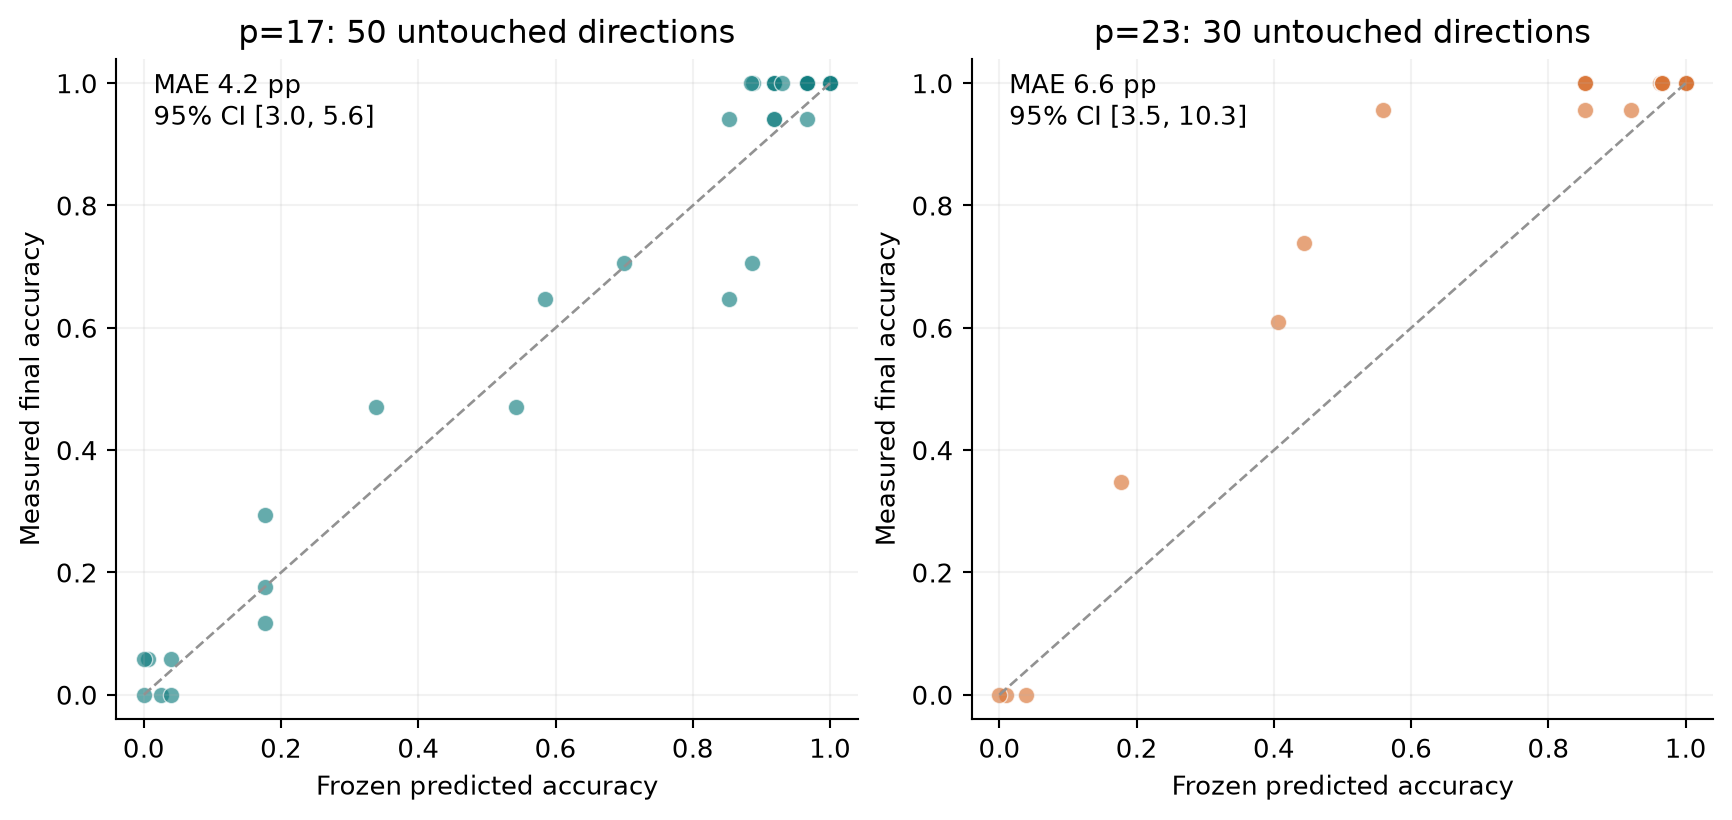
\includegraphics[width=\linewidth]{figures/02_frozen_prediction.png}
\caption{Frozen forecasts for all confirmation directions, including failures. The response bank is rebuilt for $p=23$ using the accuracy calibration fitted at $p=17$.}\label{fig:prediction}
\end{figure}

At $p=23$, threshold agreement is 83.3\%, close to the 80.0\% obtained by always predicting success. Training through step 10 and using the current accuracy gives a more accurate final-accuracy forecast than the tensor calibration on these directions. The tensor is useful here for modeling score response and selecting interventions. The experiments do not establish an overall compute saving for ordinary accuracy prediction. Earlier five-step probes gave poor forecasts and remain in the supplementary records.

\subsection{Quantization and continuous score margins}\label{sec:continuous}
The accuracy increments are $100/17=5.88$ and $100/23=4.35$ pp. In a post hoc error audit, the forecast MAEs correspond to 0.72 and 1.51 test-point increments. Errors are within one increment for 37/50 and 22/30 directions, respectively, but their 90th percentiles are 11.24 and 17.44 pp and their maxima are 20.59 and 39.73 pp. These tails matter even when the mean error is small. Changing the success threshold from 0.80 to 0.95 changes agreement from 48/50 to 43/50 at $p=17$ and from 29/30 to 24/30 at $p=23$. Appendix~\ref{app:revision} reports intermediate thresholds.

As a continuous second outcome, define the margin of the centered aligned mean profile as $m(\bar v)=\bar v_0-\max_{c\ne0}\bar v_c$. Its frozen prediction is $m(\widehat v)$. The observed MAEs are $1.88\times10^{-5}$ and $8.88\times10^{-5}$ in raw score units, with Spearman correlations 0.9995 and 0.9960. For the RMS-normalized margin, MAEs are 0.0208 and 0.0586. These statistics measure score-response prediction; they do not remove the difficulty of mapping scores to quantized accuracy. In particular, $m(\bar v)$ is not the mean of the per-test-point margins, since averaging and taking a maximum do not commute. Both quantities are released per direction.

\subsection{Changing signs at fixed spectral amplitudes}
Unmodified directions have mean accuracy 75.33\%. Favorable signs give 97.65\%, unfavorable signs 4.04\%, and removal of the circulant component 3.71\%. Within each direction, the favorable and unfavorable signs have identical per-frequency amplitudes. Their paired difference of 93.61 pp therefore occurs at fixed amplitudes and total circulant energy.

\begin{table}[t]
\centering
\caption{Paired interventions on 30 directions. The three matched controls are averaged per direction. The post hoc pooled intervals cluster by the 20 distinct integer seeds; within-modulus effects are also shown. Effects and intervals are in pp.}\label{tab:intervention}
\begin{tabular}{lrrr}
\toprule & Favorable signs & Unfavorable signs & Remove circulant\\\midrule
Mean accuracy (\%)&97.65&4.04&3.71\\
Matched control mean (\%)&85.79&79.06&75.94\\
Paired effect (pp)&+11.86&$-75.02$&$-72.23$\\
Cluster 95\% interval&[7.15, 17.03]&[$-83.68$, $-65.77$]&[$-83.99$, $-59.42$]\\
$p=17$ effect ($n=20$)&+15.69&$-69.41$&$-67.25$\\
$p=23$ effect ($n=10$)&+4.20&$-86.23$&$-82.17$\\\bottomrule
\end{tabular}
\end{table}

\begin{figure}[t]
\centering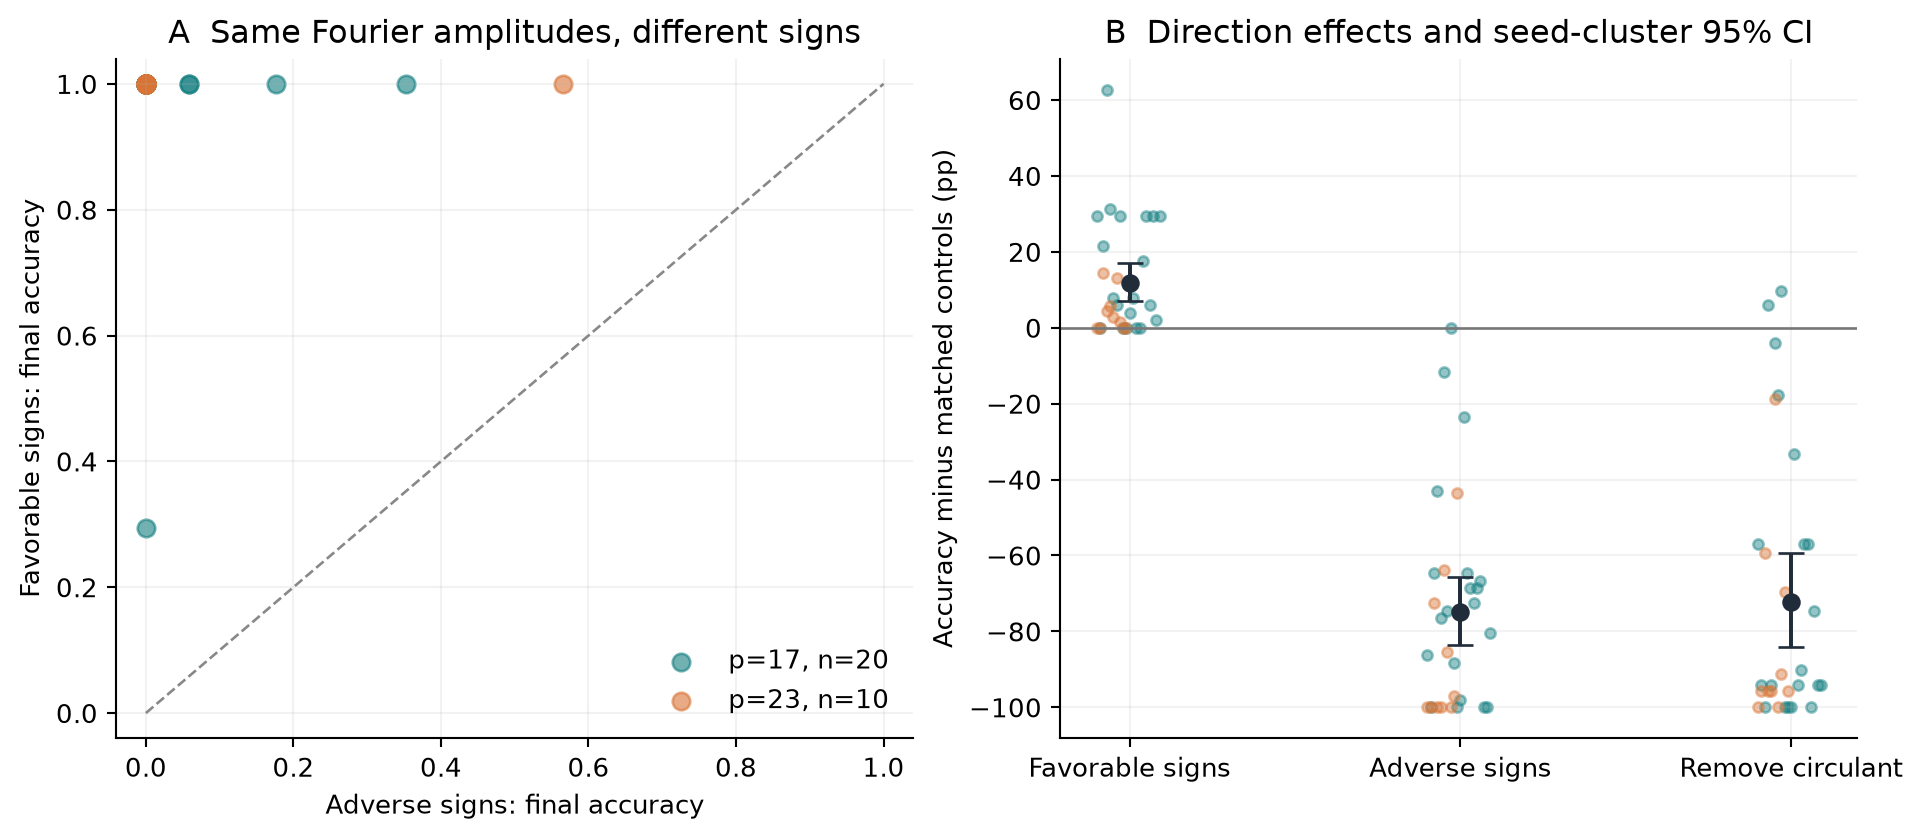
\includegraphics[width=\linewidth]{figures/03_sign_interventions.png}
\caption{Outcomes and paired effects for all prespecified intervention directions. Baselines come from confirmation. Controls match intervention distance but can change individual spectral amplitudes.}\label{fig:intervention}
\end{figure}

Compared with distance-matched controls, the mean favorable-sign improvement is 11.86 pp, with a seed-cluster bootstrap interval of [7.15, 17.03] pp. Unfavorable signs and removal produce much larger negative differences (Table~\ref{tab:intervention}). Planned direction-level Holm-adjusted Monte Carlo sign-flip values for the three pooled contrasts are approximately $1.5\times10^{-5}$; seed-cluster robustness values are $7.5\times10^{-5}$, $1.0\times10^{-5}$, and $1.0\times10^{-5}$ before multiplicity adjustment. The within-modulus effects are +15.69 pp at $p=17$ (20 directions; planned 95\% interval [8.92, 23.24]) and +4.20 pp at $p=23$ (10 directions; [1.30, 7.54]). Thus the pooled effect is driven mainly by $p=17$ and should not be read as a uniform cross-modulus gain. Favorable and unfavorable effects are also asymmetric: the high baseline and control accuracies leave much less room for improvement than for damage.

Only four intervention directions have baseline accuracy at most 10\%. Favorable signs rescue three to at least 90\%; the twelve associated random controls contain seven successes but are paired, not twelve independent baseline failures. Among twenty directions initially at least 90\% accurate, unfavorable signs reduce seventeen to at most 10\%, and removal does so for all twenty. Favorable signs are not sufficient for success: one $p=17$ direction remains at $5/17=29.41\%$. Figure~\ref{fig:fixedenergy} illustrates how identical spectral amplitudes can support different score profiles.

\begin{figure}[t]
\centering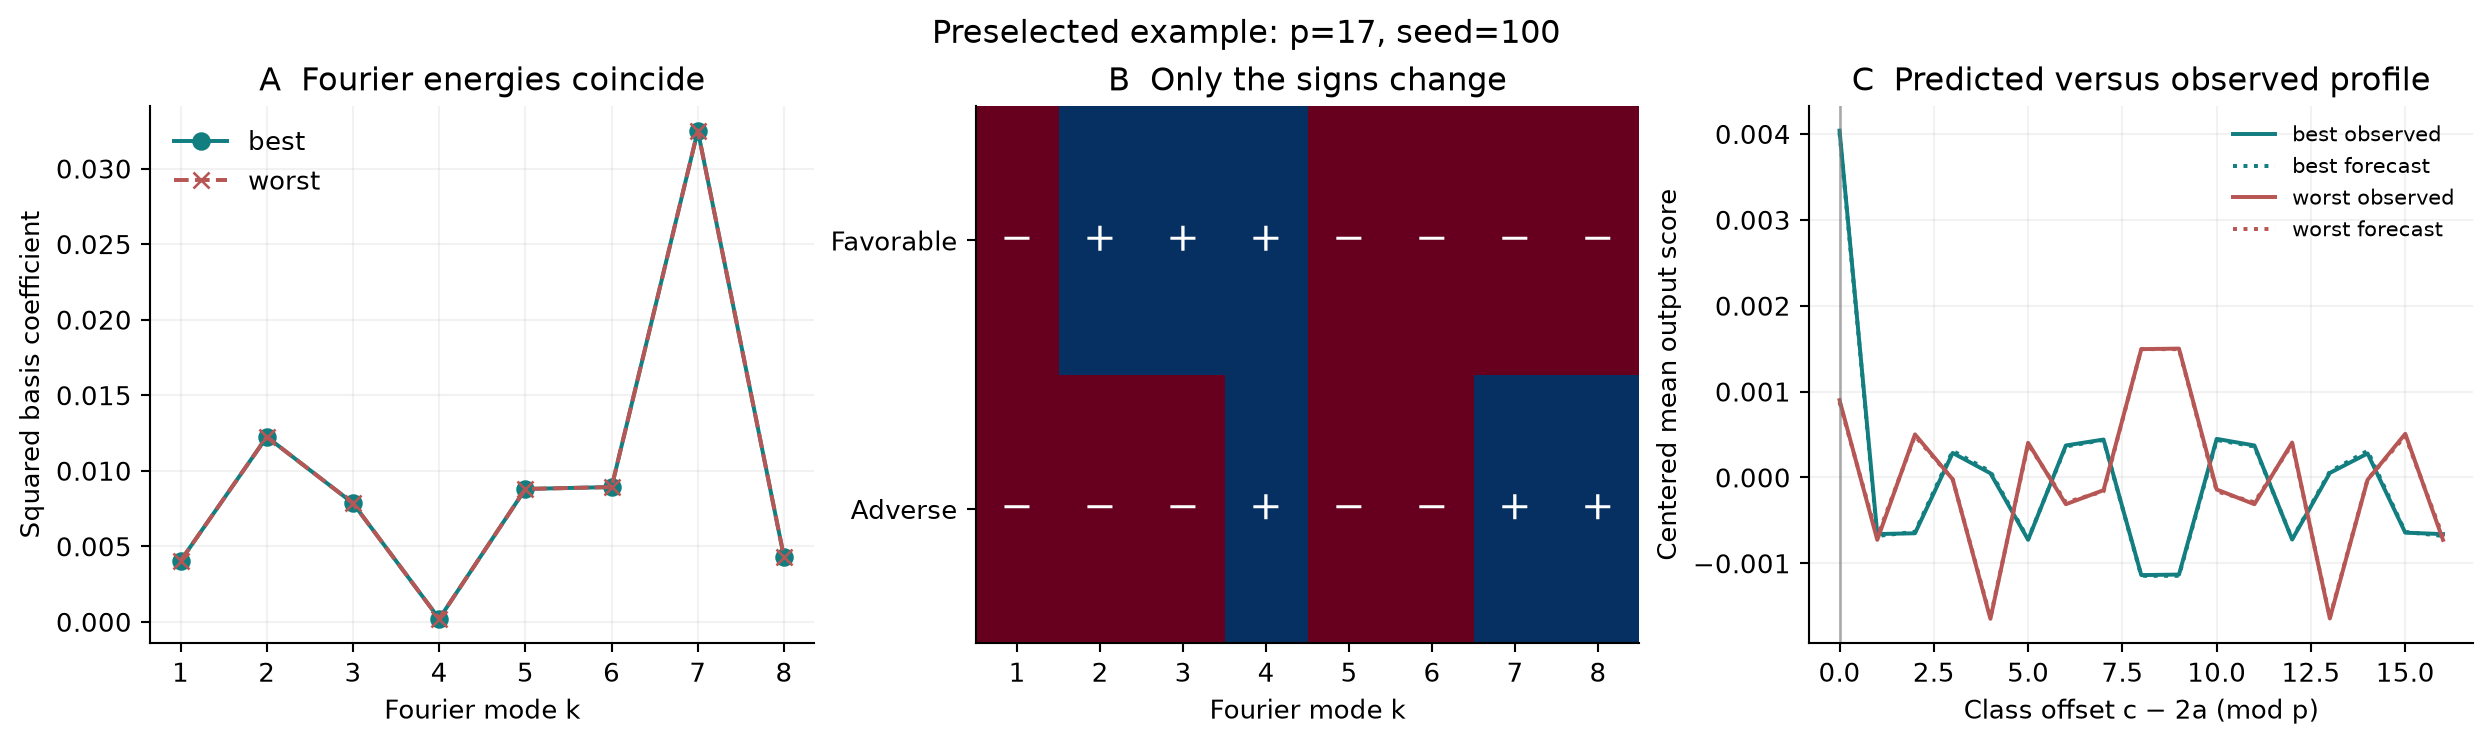
\includegraphics[width=\linewidth]{figures/05_fixed_energy_example.png}
\caption{Favorable and unfavorable signs for one prespecified direction. Fourier amplitudes coincide, while relative signs and the resulting score profiles differ.}\label{fig:fixedenergy}
\end{figure}

\subsection{Why do the matched controls also improve?}\label{sec:controlgain}
The favorable-sign controls average 85.79\%, exceeding the unmodified 75.33\% baseline by 10.46 pp. A post hoc paired audit gives an exploratory seed-cluster interval of [0.36, 21.15] pp for this control-versus-baseline difference. The corresponding within-modulus intervals include zero. At the direction level, nine control averages improve, eleven worsen, and ten are unchanged; the median change is zero. The unfavorable-sign controls instead gain 3.73 pp on average, with interval [$-3.69$, 11.19]. The data therefore do not support a general claim that any rearrangement improves a direction.

These are conditional random controls: their rotation angle is determined by an optimized sign target (Appendix~\ref{app:controls}). They are not draws from an unconditional random-reinitialization distribution, and favorable and unfavorable controls need not have the same expected outcome. Applying the unchanged tensor and calibration to the favorable controls predicts a mean gain of 12.96 pp and ranks measured direction-level gains with Spearman correlation 0.813; gain MAE is 6.05 pp. This post hoc check is consistent with a contribution from redistribution within the circulant sector, whose off-diagonal response terms depend on the coordinates.

It does not establish cancellation between circulant and residual components. The components are orthogonal in the Frobenius metric, so such a claim would have to concern nonlinear score interactions rather than cancellation of their matrix norms. The predictor uses circulant coordinates alone yet captures much of the control-gain variation. Isolating a residual interaction would require additional paired runs with and without the same residual for each rotated initializer. Those runs were not performed.

\paragraph{Unfavorable signs and chance accuracy.}
Mean unfavorable accuracy is 3.24\% at $p=17$ and 5.65\% at $p=23$, compared with uniform random-label expectations of 5.88\% and 4.35\%. These deterministic outcomes are not evidence of random guessing. In a post hoc score audit, 29/30 unfavorable mean profiles have a strictly larger incorrect-offset score than the correct score, while their RMS amplitudes are 0.48--1.08 times the paired favorable amplitudes. Their cosines with the negative favorable profile range from $-0.81$ to 0.03. Thus neither a vanished score signal nor a literal reversal of the whole favorable profile describes these cases; the observed change is primarily a loss of correct-offset dominance.

\subsection{Parameter boundaries}
For seeds 100--109 at each modulus, we evaluate eight additional settings and reuse the twenty default runs. The forecasting rule is unchanged. The default kernel convention $2\sigma^2=12.5$ differs from using the written denominator $L=2.5$ directly. We therefore evaluate this alternative explicitly, together with uncentered gradients, their combination, three bandwidths, and two perturbation amplitudes.

\begin{table}[t]
\centering
\caption{Parameter grid, ten directions per modulus per setting. Accuracy is in percent and frozen-predictor MAE in pp.}\label{tab:boundary}
\begin{tabular}{lrrrr}
\toprule &\multicolumn{2}{c}{Mean accuracy (\%)}&\multicolumn{2}{c}{MAE (pp)}\\
Setting&$p=17$&$p=23$&$p=17$&$p=23$\\\midrule
Default&60.00&83.04&4.40&4.67\\
Denominator $L=2.5$&46.47&57.83&14.99&22.10\\
Uncentered gradients&51.76&74.35&8.63&10.56\\
$L=2.5$ and uncentered&32.94&48.70&27.46&30.54\\
$\sigma=1.5$&52.35&71.30&9.79&8.62\\
$\sigma=2.0$&55.88&81.74&6.95&3.50\\
$\sigma=3.0$&62.35&84.78&2.05&6.41\\
$\epsilon=0.001$&60.00&83.04&4.40&4.67\\
$\epsilon=0.03$&62.94&83.48&2.54&5.10\\\bottomrule
\end{tabular}
\end{table}
The alternative denominator combined with uncentered gradients gives the largest tested deterioration, with MAEs of 27.46 and 30.54 pp. Accuracy at $\epsilon=0.001$ and $0.01$ coincides in this grid. This finite-sample equality leaves behavior between and beyond the tested amplitudes unresolved.

\begin{figure}[t]
\centering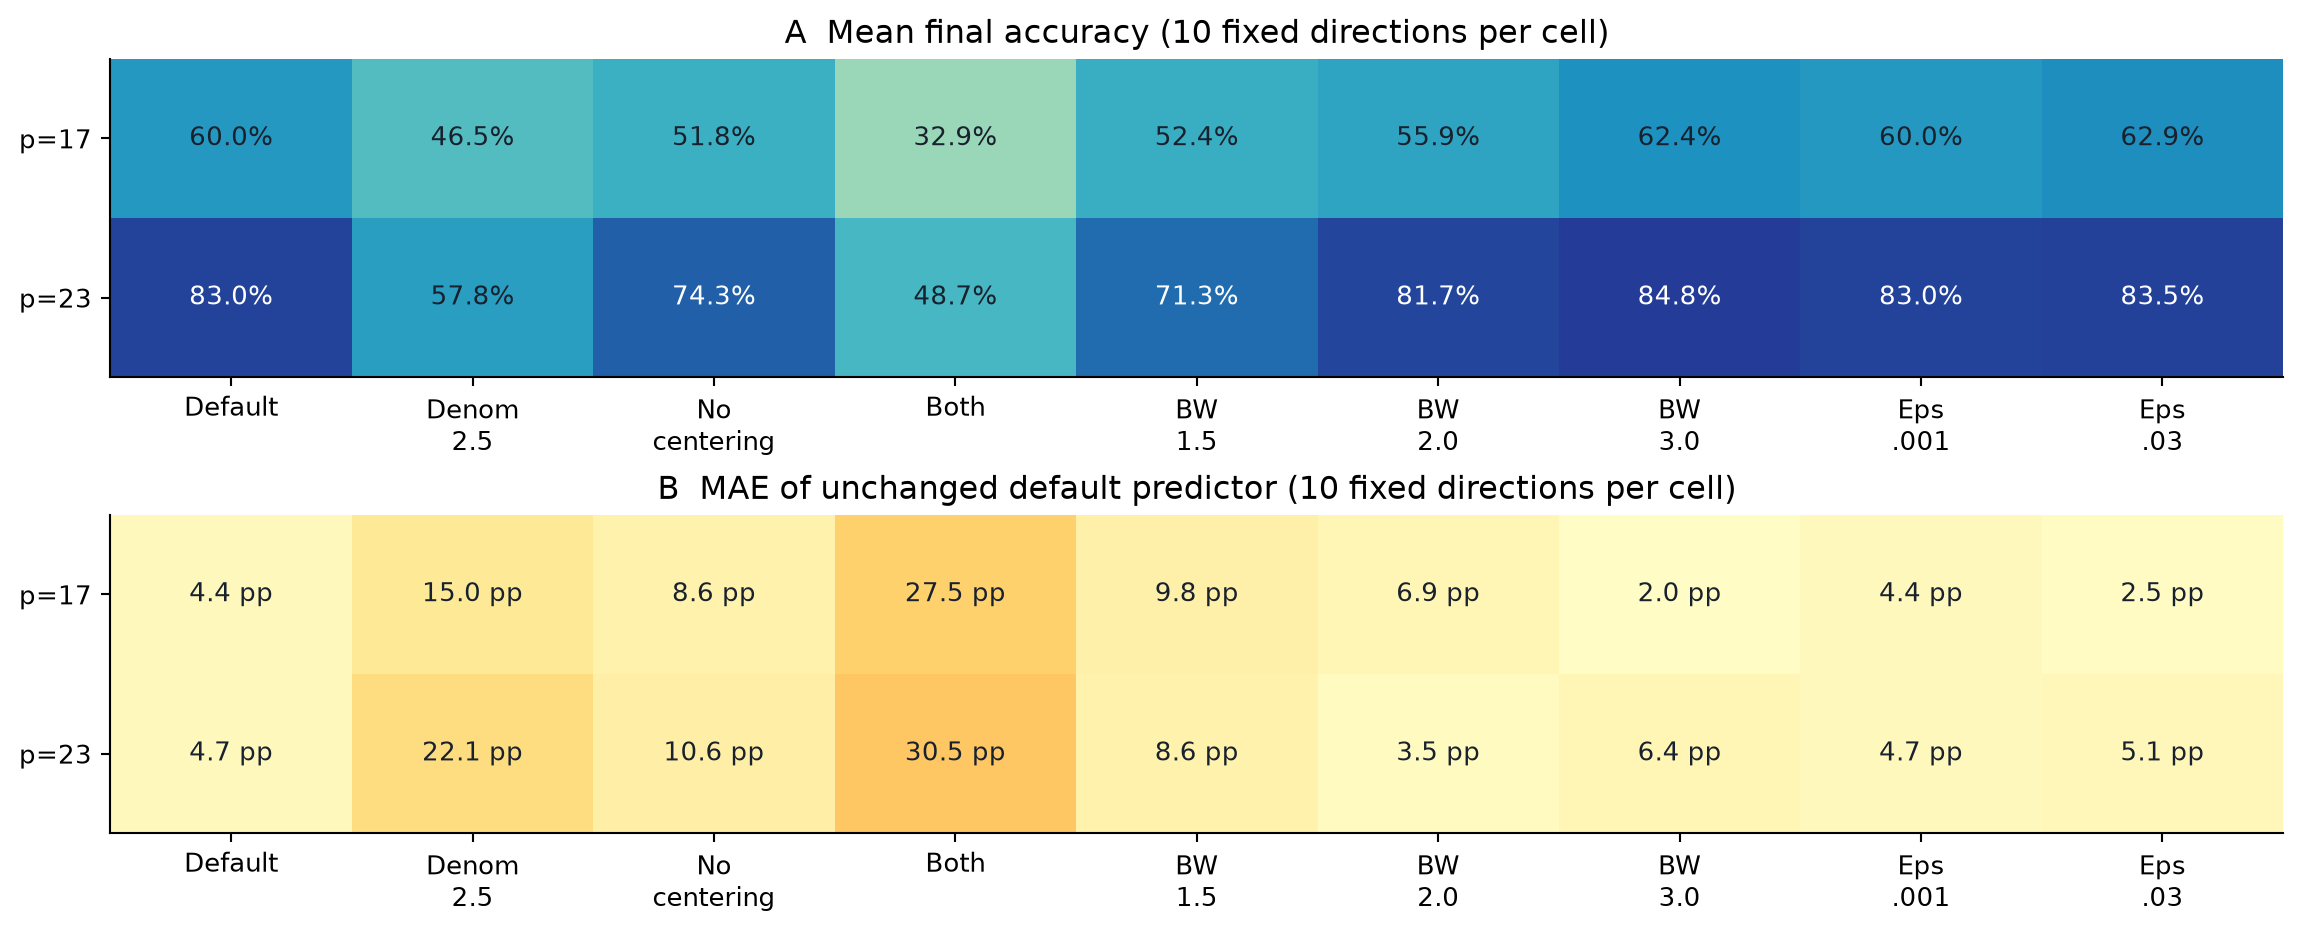
\includegraphics[width=\linewidth]{figures/04_parameter_boundaries.png}
\caption{The same frozen predictor under parameter changes. The lower panels report percentage-point errors, separating predictor deterioration from changes in the underlying final accuracy.}\label{fig:boundary}
\end{figure}

\subsection{Structure and limits of the response tensor}\label{sec:tensorstructure}
A post hoc audit finds $Q_c\simeq Q_{-c}$ to relative tensor errors $7.0\times10^{-12}$ and $5.5\times10^{-12}$, consistent with Proposition~\ref{prop:profile}. A stronger constraint comes from multiplication of every input index and output label by a nonzero residue $u$ modulo the prime $p$. Let $U_u$ be the signed permutation sending sine mode $k$ to $ku^{-1}\bmod p$, with a minus sign when folding a frequency above $(p-1)/2$ back into the sine basis. The exact pure-circulant response obeys
\begin{equation}
 V_{uc}(U_u a)=V_c(a).
\end{equation}
Consequently, if an exact quadratic coefficient $H_c$ exists at the symmetric baseline, $H_{uc}=U_uH_cU_u^T$. This is a multiplicative relabeling of offsets and a signed frequency permutation, not a cyclic translation of $c$ within one fixed initializer. All nonzero-offset $H_c$ are conjugate; $H_0$ is a separate orbit. Appendix~\ref{app:revision} gives the argument.

Our finite-amplitude $Q$ satisfies this stronger covariance only approximately: the largest relative tensor discrepancies over $u$ are 1.95\% and 6.09\%. It should therefore not be identified with an exact symmetry-constrained Hessian. Each $Q_c$ has full numerical rank at a relative eigenvalue cutoff of $10^{-8}$; retaining 95\% of squared eigenvalue mass requires 4--6 of 8 modes at $p=17$ and 6--7 of 11 at $p=23$. The off-diagonal entries account for approximately 42\% of the tensor's squared Frobenius norm. The leading unit eigenvector $w$ of $Q_0$ mixes frequencies: its participation number $1/\sum_k w_k^4$ is 3.59 and 7.54, with largest squared frequency weights 0.362 and 0.196. Near-degenerate eigenspaces can make individual eigenvectors unstable, so the complete spectra and eigenvectors are supplied rather than interpreted as unique task features. Output reflection and class centering bound the rank of the output-flattened tensor by $d$; the observed numerical ranks are exactly $d=8$ and 11, without further low-rank reduction at the 95\% energy criterion.

The additive Fourier expansion of the target identifies the correct sum, but does not by itself specify the RFM's finite-time response coefficients or their sign-interaction optimum. For comparison, the neural phase condition $2\phi-\psi=0\pmod{2\pi}$ in \citet{he2026} couples input and output phases of a two-layer network. Our $a_k$ parameterize a skew cross-metric perturbation with a different update rule. We have not derived an analogous analytic optimum from the addition table, and these experiments do not rule out a cheaper closed-form construction.

\begin{figure}[t]
\centering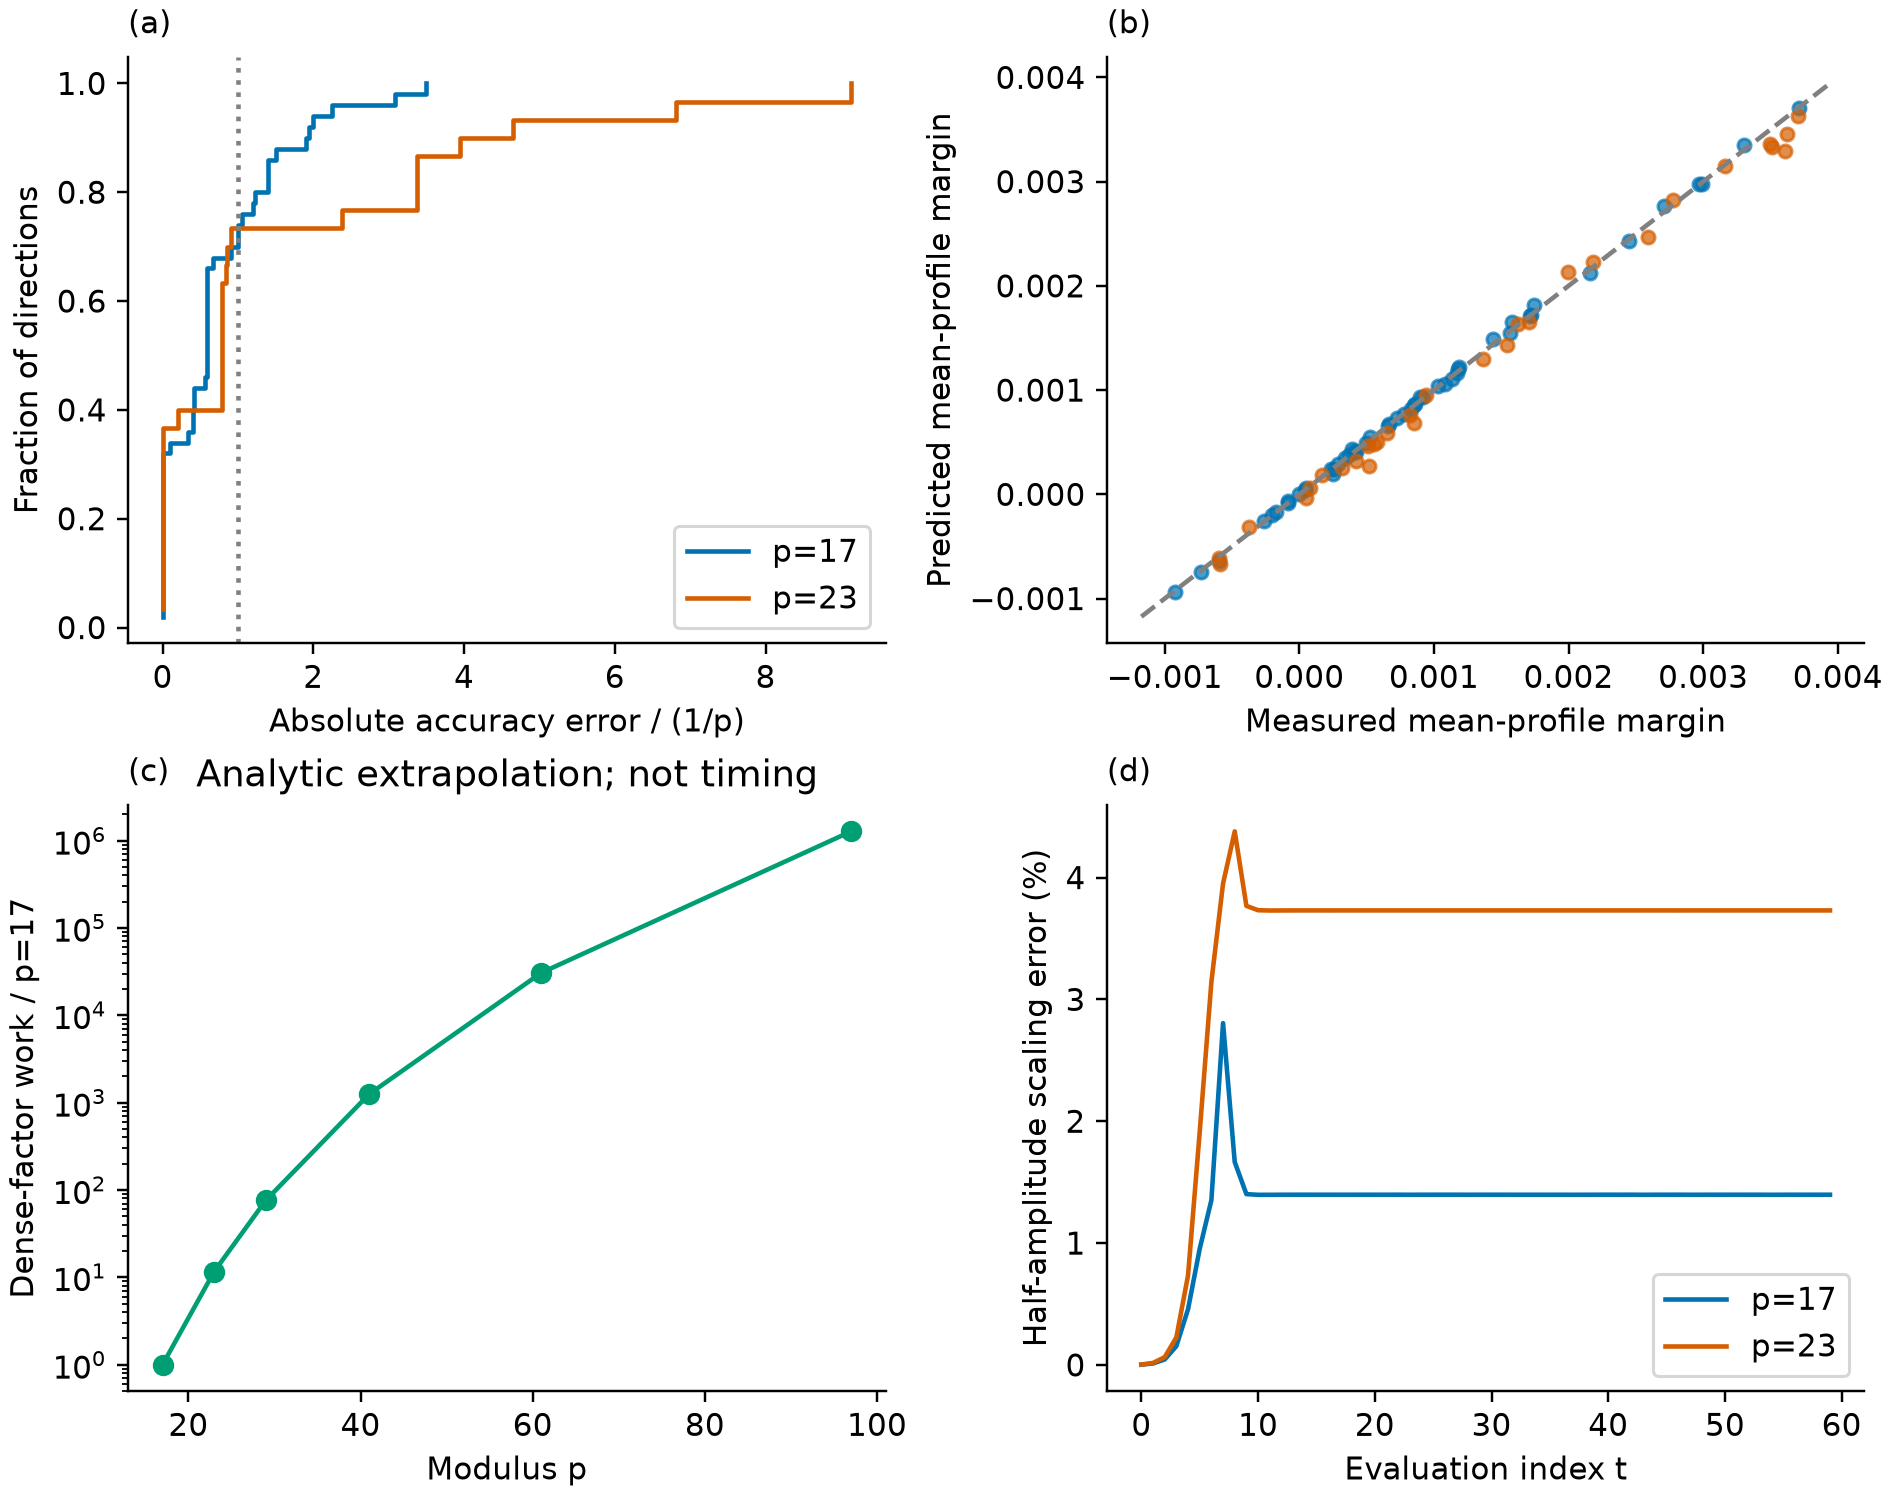
\includegraphics[width=\linewidth]{figures/06_revision_diagnostics.png}
\caption{Post hoc diagnostics. (a) Accuracy-error distribution in test-point increments. (b) Continuous mean-profile margins in raw score units. (c) Dense-factorization work extrapolated analytically from bank size and training-set size; this is not measured timing. (d) Departure from quadratic half-amplitude scaling along the stored pure mode-1 trajectories.}\label{fig:revision}
\end{figure}

\FloatBarrier
\section{Relation to prior work and limitations}\label{sec:limitations}
\citet{mallinar2025} establish grokking and block-circulant feature learning in RFMs, including structured circulant projection. \citet{bernal2026} connect data invariance groups to metric structure and recover generalization by changing initialization in Appendix F. For neural modular addition, \citet{he2026} analyze Fourier features, phase alignment, and frequency competition. \citet{gu2025} use circulant embedding initialization in Appendix E. Our work refines this existing line of research through a frozen numerical predictor and sign interventions at fixed spectral amplitudes for the RFM split.

Confirmation covers two small moduli, with $p=29$ used only in local checks. The data are synthetic, the split is deliberately structured, and calibration uses discovery test outcomes and the known modular-addition rule. Generalization to larger moduli, different splits, neural networks, or unknown tasks remains untested. Independent implementations could also expose sensitivity to the numerical choices made here.

The largest theoretical gap is why a quadratic model remains accurate after 59 nonlinear updates. Proposition~\ref{prop:even} gives evenness, and Proposition~\ref{prop:selection} constrains one local derivative; neither bounds higher-order contributions along the full trajectory. Even assuming a $C^4$ response would only yield $V(\epsilon)=\epsilon^2V_2+O(\epsilon^4)$ after centering and baseline subtraction. A useful finite-amplitude guarantee also needs a controlled remainder relative to a nonvanishing quadratic signal, including near decision boundaries. Such a bound has not been established through the singular AGOP square roots.

The saved trajectories show departures from exact quadratic homogeneity. For pure mode 1, the half-amplitude scaling discrepancy grows from 0.0020\%/0.0028\% at evaluation zero to 1.40\%/3.73\% at evaluation 59 for $p=17/23$. For ten general cross directions per modulus, rescaling the $\epsilon=0.001$ profiles by $100$ and comparing them with $\epsilon=0.01$ gives median relative errors 0.96\%/1.56\%; rescaling $\epsilon=0.03$ by $1/9$ gives 6.85\%/10.63\%. These post hoc checks support an approximate finite-amplitude description and expose its error, rather than explaining why nonlinear contributions remain small. A simpler first-fit explanation is already ruled out: diag perturbations have nonzero second-order test responses (Appendix~\ref{app:taylor}).

The rescue evidence has weak specificity: among just four baseline failures at accuracy $\le0.1$, favorable signs rescue three, while seven of their twelve paired random-control trajectories also reach $\ge0.9$. These controls show that the selected signs are not necessary for rescue, and the remaining favorable failure shows they are not sufficient. The experiments also leave open when generalization can survive circulant removal and which nonlinear pathways the tensor misses.

\paragraph{Scaling and an untested selection baseline.}
For $d=(p-1)/2$, the bank requires $B=1+d(d+1)/2$ complete trajectories, each with 60 kernel fits on $n=p(p-1)$ training points. The dense factorization contribution scales as $B n^3=O(p^8)$ for fixed trajectory length; a single FP64 kernel alone stores $8n^2$ bytes. This operation-count model omits other arrays and implementation effects and is not a wall-clock prediction. It yields bank sizes 106, 211, and 466 at $p=29,41,61$, with relative dense-factor work about 76, 1,250, and 30,685 times the $p=17$ bank. Exhaustive sign selection further costs $2^{d-1}$ candidates per direction. The numerical bank is rebuilt for each modulus; only the calibration rule was transferred. Appendix~\ref{app:revision} and Figure~\ref{fig:revision} give the cost extrapolation.

A missing intervention-selection baseline is greedy coordinate sign search using short training probes. If a probe evaluates indices 0 through 10, one sweep over the $d-1$ free relative signs, including an initial probe, costs approximately $11d$ kernel fits per direction, or $11[1+R(d-1)]$ for $R$ sweeps without caching. In contrast, building this bank costs $60B$ fits before sign scoring. Probe runs must restart from each candidate initialization to target the same intervention, and their selection accuracy must be compared on the same prespecified directions and total fit budget, reporting both one-direction and amortized costs. Step-10 accuracy works well as a forecast on the current random directions, but has not been tested as a greedy selection objective on adaptive sign candidates. No greedy-search performance or compute advantage is claimed here.

\section{Reproducibility and computational disclosure}\label{sec:repro}
Experiments ran in FP64 on an RTX 4070 under WSL, with one PyTorch CPU thread and TF32 disabled. Source code, exact plans, frozen forecasts and initializers, fitted response banks, per-direction tables, all 47,940 per-step metric records, and numerical-check reports accompany the submission as ancillary material. Appendix~\ref{app:artifacts} gives the file map and reproduction commands. The full local archive additionally contains all intermediate matrix checkpoints and score histories; the compact ancillary release explicitly inventories which large arrays it omits. The revision adds a separate post hoc analysis script, extracted score and coordinate inputs with original-file hashes, per-direction outputs, and tensor eigensystems. These additions are outside the original freeze and can be recomputed without rerunning training.

An audit recomputed saved accuracy and regression metrics for all 844 trajectories, with maximum discrepancy $1.11\times10^{-16}$, and exactly reproduced all 80 frozen forecast values. Twenty repeated earlier trajectories were bitwise identical in initialization, final metric, scores, and score history. A clean-copy smoke test reproduced two complete 60-evaluation trajectories, including one custom sign initializer, bitwise. These checks do not amount to an independent implementation or a full second execution of all 844 runs.

For sixteen stored final metrics, fixed-metric kernel readouts were repeated using extended-precision arithmetic, and two cases additionally used 50-decimal-digit LU solves. Correct prediction counts were unchanged, with maximum score difference approximately $5.43\times10^{-14}$ and measured kernel condition numbers approximately $3.5\times10^4$--$6.6\times10^4$. This audit concerns readout from symmetrized stored metrics; it is not arbitrary-precision training. Incorrect-class argmax ties are recorded rather than treated as identical outputs.

\paragraph{Code provenance.}
The base RFM implementation is adapted from the code released with \citet{bernal2026}, \url{https://github.com/marceltomas/breaking-data-symmetries}, commit \texttt{311273bfc08adcde344c8b021fc5aa8d9970ad98}. The included code retains its GPL-3.0 license and attribution. The ancillary notice distinguishes code licensing from the manuscript's arXiv distribution license.

\paragraph{Author contributions and AI assistance.}
Xiao Tian initiated and directed the study, set the research goals and computational constraints, and guided the manuscript revisions. OpenAI Codex assisted with developing the approach, mathematical analysis, implementing and running experiments, analyzing and presenting results, and manuscript preparation. Numerical results were obtained by executing the accompanying code. The computational checks were also AI-assisted and do not constitute independent validation. Xiao Tian takes responsibility for the manuscript.

\section{Conclusion}
For this fixed-point modular-addition split, favorable relative signs improve accuracy over distance-matched controls by 15.69 pp at $p=17$ (20 directions) and 4.20 pp at $p=23$ (10 directions). The pooled 11.86 pp gain summarizes unequal effects and conditional controls; the 97.6\% versus 4.0\% contrast illustrates two optimized sign extremes. The finite-amplitude tensor forecasts score profiles and selects interventions at fixed spectral amplitudes, but neither the observed gains nor approximate quadratic behavior establish a general initialization principle. Explaining the late nonlinear dynamics and comparing selection against short-probe search remain the main unresolved steps.

\bibliographystyle{plainnat}
\bibliography{references}
\clearpage
\appendix
\section{Differentiating the first update}\label{app:derivatives}
Write $M(t)=I+tE$ and $d_E(x,z)=(x-z)^TE(x-z)$. Kernel and coefficient derivatives are
\begin{equation}
 \dot K_{ij}=-K_{ij}\frac{d_E(x_i,x_j)}{2\sigma^2},\qquad
 \dot\alpha=-K^{-1}\dot K\alpha .
\end{equation}
For a point $z$, an uncentered Jacobian row for output $c$ is
\begin{equation}
 [\nabla f_M(z)]_c=\frac1{\sigma^2}\sum_j\alpha_{jc}k_M(x_j,z)M(x_j-z).
\end{equation}
Its derivative follows by differentiating $\alpha$, $k_M$, and $M$ in the product. Centering across $z=x_i$ commutes with differentiation. Thus
\begin{equation}
 \dot A=\frac1n\sum_i(\dot G_i^TG_i+G_i^T\dot G_i).
\end{equation}
If $S=A^{1/2}$ has a derivative $H$, it satisfies $SH+HS=\dot A$. In an eigenbasis of $A$, for a positive denominator,
\begin{equation}
 H_{ij}=\frac{\dot A_{ij}}{\sqrt{\lambda_i}+\sqrt{\lambda_j}}.
\end{equation}
One must not divide a zero--zero block by zero or infer full differentiability from the remaining blocks. The numerical calculation works on separated positive spectral support, sets the zero--zero block to zero, and checks the Sylvester residual. At the checked initial baselines there are two null modes, with the remaining eigenvalues separated from zero. Analytic Sylvester residuals are approximately $10^{-15}$; finite-difference discrepancies are approximately $10^{-5}$ and are affected by floating-point square roots near null eigenvalues. Detailed eigenvalues, gains, leakage, and residuals are retained in \texttt{linear\_checks.json} and \texttt{modes.json}. These are checks of the stated local calculation, not a proof of smoothness at all subsequent singular metrics.

\section{A rejected first-fit explanation}\label{app:taylor}
Even test readout does not imply that its first nonzero response belongs exclusively to cross perturbations. Expand the training kernel and the train-to-test kernel as $K_0+\epsilon K_1+\epsilon^2K_2+\cdots$ and $Z_0+\epsilon Z_1+\epsilon^2Z_2+\cdots$. With coefficients defined without factorials,
\begin{align}
 \alpha_0&=K_0^{-1}Y,\\
 \alpha_1&=-K_0^{-1}K_1\alpha_0,\\
 \alpha_2&=K_0^{-1}(K_1K_0^{-1}K_1-K_2)\alpha_0,\\
 F_2&=Z_2^T\alpha_0+Z_1^T\alpha_1+Z_0^T\alpha_2.
\end{align}
The last expression contains diag, cross, and mixed contributions. For $p=17$, seed 20, the measured second-order coefficient norm after removing the per-class component constant across test points is approximately 8.11 for diag and 4.64 for cross. The diag contribution is neither zero nor smaller in this example. The selection rule concerns the metric update's allowed linear sectors, which is a different statement from exclusivity of the first fit's quadratic readout.

\section{Intervention matching and uncertainty}\label{app:controls}
Let $a\in\R^d$ denote the circulant coordinates, $r=\norm{a}_2$, and $b$ a selected sign vector, so $\norm{b}_2=r$. Let $u=a/r$ and $\gamma=a^Tb/r^2$. Draw a random unit vector $w$ orthogonal to $u$ in the circulant coordinate space and set
\begin{equation}
 a_{\rm ctrl}=r\left(\gamma u+\sqrt{1-\gamma^2}\,w\right).
\end{equation}
Then $\norm{a_{\rm ctrl}}_2=r$ and $\norm{a_{\rm ctrl}-a}_2=\norm{b-a}_2$. Keeping $E_R$ unchanged also preserves the full perturbation norm and matches full-matrix displacement. Three independent deterministic-seed draws are recorded for each favorable and unfavorable intervention. Unlike the sign intervention, these controls redistribute amplitudes between circulant frequencies.

For removal, $E_{\rm remove}=E_R/\norm{E_R}_{\Frob}$. A random unit vector in the full cross sector, orthogonal to the original $E$, is combined with $E$ at the angle $\langle E,E_{\rm remove}\rangle_{\Frob}$, giving a normalized distance-matched control. These controls retain neither the original residual nor its circulant energy; their purpose is to distinguish removal from an arbitrary equal-size perturbation. The two control families therefore answer different questions and should not be conflated.

For each direction, the measured contrast is the structured outcome minus the mean of its three controls. Pooled means weight directions equally, giving weights $20/30$ and $10/30$ to the two moduli. The supplementary tables retain individual control outcomes. Seed-cluster bootstrap sampling resamples integer seeds with all their associated modulus observations to check sensitivity to shared random-number seeds.

\section{Post hoc diagnostics and analytic cost accounting}\label{app:revision}
All analyses in this appendix and Sections~\ref{sec:continuous}, \ref{sec:controlgain}, and \ref{sec:tensorstructure} were added after the frozen confirmation. They reuse saved results and do not create further independent observations. New control-gain intervals use 10,000 paired integer-seed cluster bootstrap resamples with seed 20260907 and no multiplicity adjustment; they are exploratory. Within each modulus, clustering reduces to resampling directions. The earlier pooled intervention interval in the abstract is the separately recorded post hoc robustness interval, with the original analysis seed 20260906.

\paragraph{Unit relabeling.}
For a unit $u$ modulo prime $p$, permuting both input indices by $u$ preserves equality and inequality of input pairs and permutes label $c$ to $uc$. The isotropic baseline, Gaussian kernel, and AGOP-root update are equivariant under this permutation whenever their solutions are unique. A sine block with entries $\sin(2\pi k(j-i)/p)$ is sent to mode $ku^{-1}$, giving the signed permutation $U_u$. The fixed test point $(0,0)$ is unchanged and its output labels are permuted, so $V_{uc}(U_u a)=V_c(a)$ at every defined iterate. Comparing quadratic coefficients, if they exist, gives $U_u^TH_{uc}U_u=H_c$. The audit measures $\big(\sum_c\|Q_{uc}-U_uQ_cU_u^T\|_F^2/\sum_c\|Q_c\|_F^2\big)^{1/2}$ over all nonzero $u$, including the identity. Finite-amplitude polarization need not inherit exact Hessian identities. Output reflection leaves $d+1$ independent offsets; subtracting the class mean leaves at most $d$ independent output rows.

\paragraph{Continuous margins and amplitude scaling.}
For aligned scores $S_{a,c}=F(a,a)_{c+2a}$, the pointwise mean margin is $p^{-1}\sum_a[S_{a,0}-\max_{c\ne0}S_{a,c}]$, while the profile margin is $\bar v_0-\max_{c\ne0}\bar v_c$. The latter is at least the former by convexity of the maximum. Their mean observed gaps are $1.39\times10^{-4}$ and $1.19\times10^{-4}$, so they should not be substituted for one another. The half-amplitude discrepancy at step $t$ is $\|4V_t(0.001)-V_t(0.002)\|_2/\|V_t(0.002)\|_2$ for the stored mode-1 probes, with the corresponding symmetric baseline subtracted. General-cross comparisons use centered aligned profiles at evaluation 59 and the $0.01$ profile as reference. They test homogeneity on a finite grid, not convergence to an infinitesimal Hessian.

\begin{table}[ht]
\centering
\caption{Post hoc threshold sensitivity. Counts compare frozen predicted and observed accuracy; required correct counts account for the discrete test set.}\label{tab:thresholds}
\begin{tabular}{crrrr}
\toprule Threshold &\multicolumn{2}{c}{$p=17$, 50 directions}&\multicolumn{2}{c}{$p=23$, 30 directions}\\
 &Required correct&Agreement&Required correct&Agreement\\\midrule
0.80&14/17&48/50&19/23&29/30\\
0.85&15/17&48/50&20/23&29/30\\
0.90&16/17&47/50&21/23&25/30\\
0.95&17/17&43/50&22/23&24/30\\\bottomrule
\end{tabular}
\end{table}

\begin{table}[ht]
\centering
\caption{Analytic cost extrapolation, not measured timing or peak memory. Bank trajectories exclude validation probes; memory covers only one dense kernel.}\label{tab:cost}
\begin{tabular}{rrrrrr}
\toprule $p$&$n$&$B$&$Bn^3$ / $p=17$&Kernel GiB&Sign candidates\\\midrule
17&272&37&1&0.00055&$2^7$\\
23&506&67&11.7&0.00191&$2^{10}$\\
29&812&106&76.2&0.00491&$2^{13}$\\
41&1,640&211&1,250&0.0200&$2^{19}$\\
61&3,660&466&30,685&0.0998&$2^{29}$\\
97&9,312&1,177&1,276,430&0.646&$2^{47}$\\\bottomrule
\end{tabular}
\end{table}
\FloatBarrier

\section{Artifact map and reproduction}\label{app:artifacts}
The ancillary package contains the following relative paths. It preserves the executed source and frozen plans; publication packaging is recorded separately.
\begin{itemize}
\item \texttt{src/}, \texttt{vendor/}, \texttt{requirements.txt}: experiment, analysis, plotting, and numerical-check code with upstream attribution.
\item \texttt{frozen/}: forecast values, confirmation and intervention plans, parameter plans, source hashes, and the local freeze manifest.
\item \texttt{models/}, \texttt{initializations/}: response tensors, calibration, and every selected intervention matrix.
\item \texttt{results/all\_runs.csv} and \texttt{results/all\_steps.csv}: all 844 configurations/outcomes and 47,940 per-step records.
\item \texttt{results/confirmation.csv}, \texttt{intervention.csv}, and \texttt{boundary.csv}: direction-level forecast, paired comparison, and parameter-grid tables.
\item \texttt{results/}: analysis reports, local derivative and Taylor checks, and fixed-metric precision checks. Run-level configuration and summary files retain individual failures and outcomes.
\item \texttt{revision/}: post hoc analysis code, extracted inputs, provenance hashes, direction-level diagnostics, tensor spectra, and the analytic cost table.
\item \texttt{PUBLICATION\_README.md}, \texttt{PUBLICATION\_MANIFEST.json}: exact inclusion/omission inventory, checksums, and commands for the compact release.
\end{itemize}
With the recorded dependencies installed and a compatible CUDA-enabled PyTorch build, full regeneration writes to a new directory:
\begin{verbatim}
python src/reproduce.py --phase all --output /path/to/new-run
\end{verbatim}
The corresponding smoke command is
\begin{verbatim}
python src/reproduce.py --phase smoke --output /path/to/new-smoke
\end{verbatim}
It compares one ordinary cross and one custom-initialization trajectory to the included reference arrays. The programs refuse to overwrite an existing output directory. Hardware or numerical-library changes can alter floating-point tie breaking; bitwise agreement is only claimed for the checked environment. A separate lightweight publication check recomputes counts, accuracy means, MAEs, and paired effects directly from the released CSV files without rerunning training. The post hoc diagnostics require NumPy, SciPy, and Matplotlib and can be recomputed from the ancillary root with
\begin{verbatim}
python revision/revision_analysis.py --inputs revision/inputs 
    --output /path/to/new-diagnostics
\end{verbatim}
The command is shown wrapped for typesetting; enter it on one line. Input hashes distinguish the original frozen study from the revision's extracted arrays.
\end{document}
